%Template by Mark Jervelund - 2015 - mjerv15@student.sdu.dk

\documentclass[a4paper,10pt,titlepage]{report}

\usepackage[utf8]{inputenc}
\usepackage[T1]{fontenc}
\usepackage[english]{babel}
\usepackage{amssymb}
\usepackage{amsmath}
\usepackage{amsthm}
\usepackage{graphicx}
\usepackage{fancyhdr}
\usepackage{lastpage}
\usepackage{listings}
\usepackage{algorithm}
\usepackage{algpseudocode}
\usepackage{MnSymbol}
\usepackage[document]{ragged2e}
\usepackage[margin=1in]{geometry}
\usepackage{color}
\usepackage{datenumber}
\usepackage{venndiagram}
\usepackage{chngcntr}
\usepackage{enumitem}
\usepackage{mathtools}
\usepackage{tikz}
\usetikzlibrary{automata,positioning}
\DeclarePairedDelimiter{\ceil}{\lceil}{\rceil}

\title{DM553 - Notes}


\setdatetoday
\addtocounter{datenumber}{0} %date for dilierry standard is today
\setdatebynumber{\thedatenumber}
\date{}
\setcounter{secnumdepth}{0}
\pagestyle{fancy}
\fancyhf{}

\newcommand{\Z}{\mathbb{Z}}
\lhead{Complexity and Computability (DM553 - Notes))}
\rhead{Mark Jervelund (Mjerv15)}
\rfoot{Page  \thepage \, of \pageref{LastPage}}
\counterwithin*{equation}{section}

\begin{document}





\renewcommand{\thepage}{\roman{page}}% Roman numerals for page counter
\tableofcontents
\newpage
\setcounter{page}{1}
\renewcommand{\thepage}{\arabic{page}}
\section{Course description}
%%%%%%%%%%%%%%%%%%%%%%%%%%%%%%%%%%%%%%%%%%%%%
\newpage

\chapter{Questions 2018}
\newpage
\section{1. Finite automata and regular languages}

Introduction
What is it

Finite atomata

Nondetermanistic


NFA
DFA


Pumping lemma for regular languages






\newpage
\section{2. Pushdown automata and context-free languages}

%Chomsky normal form.


What is a push down

What is a context free grammar
a -> 0a1
A -> B
B -> #
    ambiguity
    grammar
    variables


What can it be used to
    programming languages
    Compiler
    
    

        
Pushdown atomata in dept
    You use a stack.
    
Pumping lemma
    Proof
    
    Application
    



\newpage
\section{3. Turing machines}

Introduction
    What is a turning machine
        
Multitape

Nondetermanistic turning machine
    Faster but less powerfull?
    



\newpage
\section{4. Decidability}
Introduction
 If a language  defined by a DFA is decidable.


Examples of Decidability and undecidability




\newpage
\section{5. Reducibility}
What is it and how to use it.





\newpage
\section{6. NP-completeness proofs – examples.}
what is np_completeness

Why we use it to reduce,

Proff of np complete.
qlique, subset sum, Hamiltonian circuit, 




\newpage
\section{7. Proof that SATISFIABILITY is NP-complete (do not assume that
there is a known NP-Complete problem — use the proof in Sipser’s
book).}

Cook-levin theorem - insipset, præsentation use slides on homepage.
\newpage
\section{8. Information-theoretic lower bounds (lower bounds proven by counting
leaves in decision trees), especially the average case bounds for sorting
by comparisons.}
As is average case.




\newpage
\section{9. Adversary arguments – technique, examples.}





\newpage
\section{10. Median problem – algorithm and lower bound.}





\newpage
\section{11. Approximation algorithms}













%%%%%%%%%%%%%%%%%%%%%%%%%%%%%%%%%%%5
\newpage
\chapter{Questions 2017}
\section{Questions from last year}
1. Finite automata and regular languages \\
2. Pushdown automata and context-free languages\\
3. Turing machines\\
4. Decidability\\
5. Reducibility\\
6. NP-completeness proofs – examples.\\
7. Proof that SATISFIABILITY is NP-complete.\\
8. Information-theoretic lower bounds (lower bounds proven by counting leaves in decision trees), especially the average case bounds for  sorting by comparisons.\\
9. Adversary arguments – technique, examples.\\
10. Approximation algorithms.\\
\newpage
\subsection{1. Finite automata and regular languages}
\subsubsection{Introduction}
\subsubsection{Types of Automata}
	DFA - 
    NDFA - 

\newpage
\subsection{2. Pushdown automata and context-free languages}
	CFG(context free grammar)
    	regular language
        	defined by DFA
           ambiguity
           		inherited ambiguity
           Chomsky normal form
           		You're allowed to have a rule that turns A into two sub rules.
           			A -> BC
                You can have a rule about a terminal set for our alphabet.
                	$A -> a \in \sum \epsilon $
                You're only allowed to produce Epsilon from the start symbol.
                	$S -> \epsilon $
            theorem
            	Any CFL is generated by a CFG in Chomsky normal form,
                
    pushdown automata PDA(s) 
    		NFA with a stack.
    	
    	
           
\subsection{3. Turing machines}
\subsection{4. Decidability}
\subsection{5. Reducibility}
\subsection{6. NP-completeness proofs – examples.}
\subsection{7. Proof that SATISFIABILITY is NP-complete.}
\subsection{8. Information-theoretic lower bounds (lower bounds proven by counting leaves in decision trees), especially the average case bounds for sorting by comparisons.}
\subsection{9. Adversary arguments – technique, examples.}
\subsection{10. Approximation algorithms}

\newpage
\chapter{Lectures}
\subsection{Format}
Titles should be listed as (date - topic(s)) for easier lookup

\subsection{28-feb-2018 - TBD}
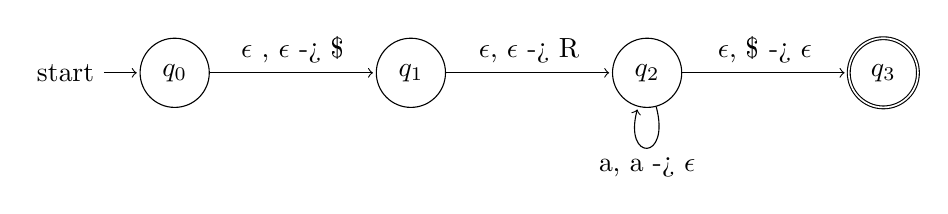
\begin{tikzpicture}[shorten >=1pt,node distance=3cm,on grid,auto] 
   \node[state,initial] (q_0)   {$q_0$}; 
   \node[state] (q_1) [right=of q_0] {$q_1$}; 
   \node[state] (q_2) [right=of q_1] {$q_2$}; 
   \node[state,accepting](q_3) [right=of q_2] {$q_3$};
    \path[->] 
    (q_0) edge  node {$\epsilon$ , $\epsilon$ -> \$} (q_1)
    (q_1) edge  node {$\epsilon$, $\epsilon$ -> R} (q_2)
    (q_2) edge  node {$\epsilon $, \$ -> $ \epsilon $} (q_3) 
          edge [loop below] node {
          a, a -> $\epsilon$} (); 
\end{tikzpicture}


\section{22 march }
\subsection{assignment 2}
We can reconnize that it is two regular languages, and that when we concatinate them we get a reglang\\
sigma star is regular, \\
we can apply theom 1.49 regular langs are closed under concat.\\
\subsection{assignemnt 3}


d)\\
	use p from pumping lemma \\
    $(xy)^{3p}(x)^p$ \\
     q

\subsection{assignemnt 5}
a)
	prove by counter exsample
    \\
    ${a^ib^ic^i | i \geq 0} \cup {a,b,c}^* $
b)
	prove by counter exsample
	${a^ib^ic^i | i \geq 0} \cup {\emptyset}$
    
    


\section{10th of April}
\begin{itemize}
\item Polynomial time reductions
\item NP-completeness
\item Examples of proofs
\begin{itemize}
\item 3-SAT
\item CLIQUE
\item Vertex cover
\item Independent set
\end{itemize}
\end{itemize}


\newpage
\section{12th of April}
\subsection{CNE-SAT is NP-Complete}
\subsubsection{Cook-lenin thm}
SAT is NP-Complete\\
 	Show that:\\
    \begin{equation}
    \forall A \in NP : A \leq_p SAT,
    \end{equation}
$ A \in NP $, Let N be a polytime NTM which accepts it in time $d_1n^k +d_2$ \\
\begin{equation}
N = (Q,\sum,R, \alpha, q_o, q_accept, q_reject).
\end{equation}
Let $W = W_1W_z*W_n$ be input to A,\\
Crate (in  polytime) a boolean formula F which is satisfiable if W is accepted by N,\\
Look at accepting breach of computation tree\\
Look at sequence of configurations.
    
\subsection{Subset-sum is NP-Complete}
   
\section{17th of April}
Hamiltonian circuit is NP-complete
\\
Conclusion on NP-complete
\\
Information on theoretic lower bound technique.

\section{1st of may}
    Approximation algorithms
    \\
    $\delta$-TSP has 2-approximation algs
    \\
    For general TSP and a fixed P, $\Delta $an alg with approx p
    \\
    Vertex cover has a 2-approx alg.
 
\end{document}

